The next part is based on these \href{https://docs.google.com/presentation/d/1U1lB5bhscjbxEuH5FcFwMl5xbHl0qIEkMf5rm0MO8uE/edit#slide=id.p}{slides}. Today, we want to talk about why we are computing derivatives in the first place. In particular, we will drill down on this a little bit and then talk about computation of derivatives.

\subsection{Newton's Method}
\label{sec:newton-roots}

One common application of derivatives is to solve nonlinear equations via linearization. 

\subsubsection{Scalar Functions}

For instance, suppose we have  a scalar function $f: \R \to \R$ and we wanted to solve $f(x) = 0$ for a root~$x$. Of course, we could solve such an equation explicitly in simple cases, such as when $f$ is linear or quadratic, but if the function is something more arbitrary like $f(x) = x^3 - \sin (\cos x)$ you might not be able to obtain closed-form solutions. However, there is a nice way to obtain the solution approximately to any accuracy you want, as long if you know approximately where the root is. The method we are talking about is known as \emph{Newton's method}, which is really a linear-algebra technique. It takes in the function and a guess for the root, approximates it by a straight line (whose root is easy to find), which is then an approximate root that we can use as a new guess. In particular, the method (depicted in Fig.~\ref{fig:newton-step}) is as follows: 
\begin{itemize}
    \item Linearize $f(x)$ near some $x$ using the approximation 
    \[
    f(x + \delta x) \approx f(x) + f'(x) \delta x,
    \]
    \item solve the linear equation $f(x) + f'(x) \delta x = 0 \implies \delta x = -\frac{f(x)}{f'(x)}$,
    \item and then use this to update the value of $x$ we linearized near---i.e.,~letting the new $x$ be $$x_\text{new} = x - \delta x = x + \frac{f(x)}{f'(x)} \, .$$
\end{itemize}
Once you are close to the root, Newton's method converges amazingly quickly.  As discussed below, it asymptotically \emph{doubles} the number of correct digits on every step!

One may ask what happens when $f'(x)$ is not invertible, for instance here if $f'(x) = 0$. If this happens, then Newton's method may break down! See \href{https://en.wikipedia.org/wiki/Newton%27s_method#Failure_analysis}{here} for examples of when Newton's method breaks down.

\begin{figure}
    \centering
    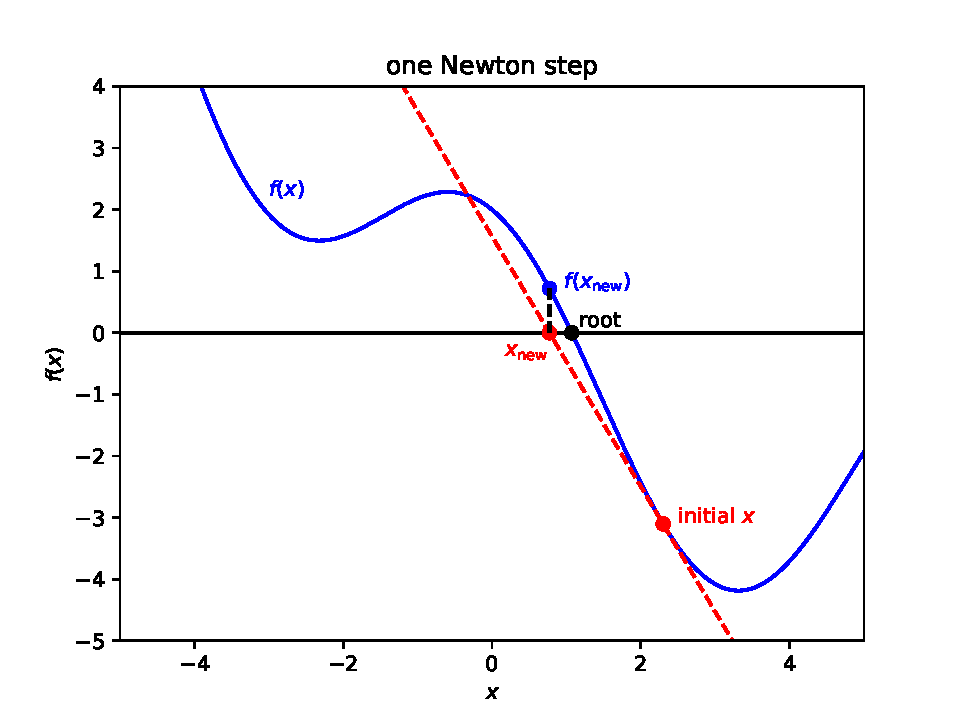
\includegraphics[width=0.7\textwidth]{figures/newton-step}
    \caption{Single step of the scalar Newton's method to solve $f(x)=0$ for an example nonlinear function $f(x) = 2\cos(x) - x + x^2/10$.  Given a starting guess ($x = 2.3$ in this example), we use $f(x)$ and $f'(x)$ to form a linear (affine) approximation of $f$, and then our next step $x_\mathrm{new}$ is the root of this approximation.  As long as the initial guess is not too far from the root, Newton's method converges extremely rapidly to the exact root (black dot).}
    \label{fig:newton-step}
\end{figure}

\subsubsection{Multidimensional Functions}
We can generalize Newton's method to multidimensional functions! Let $f: \R^n \to \R^n$ be a function which takes in a vector and spits out a vector of the same size~$n$. We can then apply a Newton approach in higher dimensions: 
\begin{itemize}
    \item Linearize $f(x)$ near some $x$ using the first-derivative approximation 
    \[
    f(x + \delta x) \approx f(x) + \underbrace{f'(x)}_\text{Jacobian} \delta x,
    \]
    \item solve the linear equation $f(x) + f'(x) \delta x = 0 \implies \delta x = -\underbrace{f'(x)^{-1}}_\text{inverse Jacobian} f(x)$,
    \item and then use this to update the value of $x$ we linearized near---i.e.,~letting the new $x$ be $$x_\text{new} = x_\text{old} - f'(x)^{-1}f(x)\, .$$
\end{itemize}

That's it! Once we have the Jacobian, we can just solve a linear system on each step. This again converges amazingly fast, doubling the number of digits of accuracy in each step. (This is known as ``quadratic convergence.'') However, there is a caveat: we \textit{need} some starting guess for $x$, and the guess needs to be sufficiently close to the root for the algorithm to make reliable progress. (If you start with an initial $x$ far from a root, Newton's method can fail to converge and/or it can jump around in intricate and surprising ways---google ``Newton fractal'' for some fascinating examples.) This is a widely used and very practical application of Jacobians and derivatives!

\subsection{Optimization}

\subsubsection{Nonlinear Optimization}
A perhaps even more famous application of large-scale differentiation is to nonlinear optimization. Suppose we have a scalar-valued function $f: \R^n \to \R$, and suppose we want to minimize (or maximize) $f$. For instance, in machine learning, we could have a big neural network (NN) with a vector $x$ of a million parameters, and one tries to minimize a ``loss'' function $f$ that compares the NN output to the desired results on ``training'' data. The most basic idea in optimization is to go ``downhill'' (see diagram) to make $f$ as small as possible. If we can take the gradient of this function $f$, to go ``downhill'' we consider $- \nabla f$, the direction of \emph{steepest descent}, as depicted in Fig.~\ref{fig:steepest-descent}. 
    \todo{It would be nice if all the ``dots" were on contours, and we can see the tangents and normals to the contours}

\begin{figure}
    \centering
    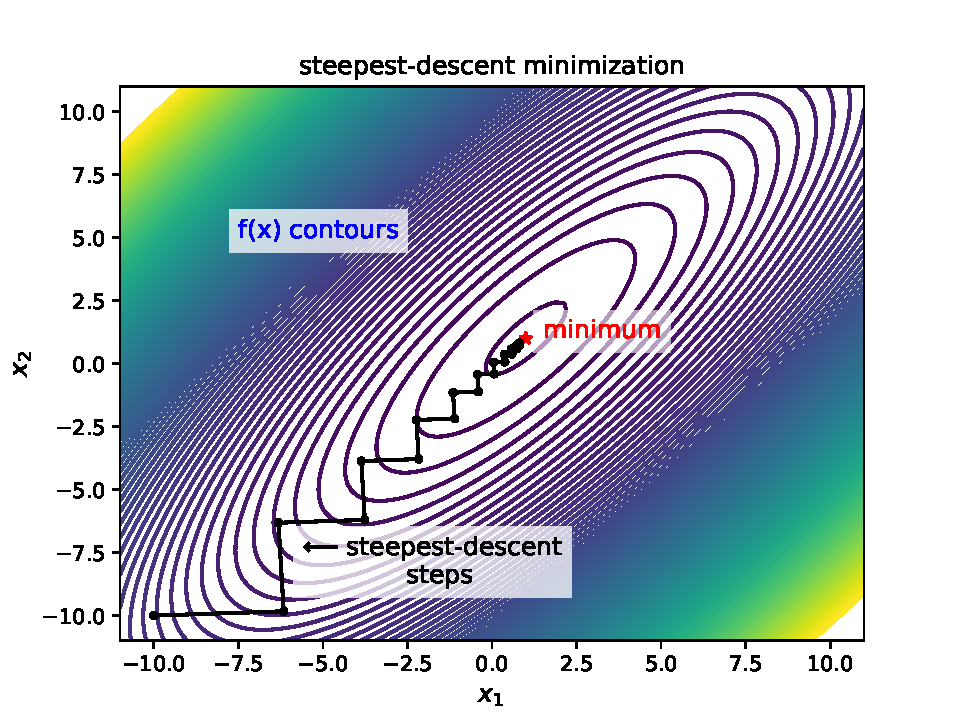
\includegraphics[width=0.7\textwidth]{figures/steepest-descent}
    \caption{    
    A \emph{steepest-descent algorithm} minimizes a function $f(x)$ by taking successive ``downhill'' steps in the direction $-\nabla f$.  (In the example shown here, we are minimizing a quadratic function in two dimensions $x \in \mathbb{R}^2$, performing an exact 1d minimization in the downhill direction for each step.)  Steepest-descent algorithms can sometimes ``zig-zag'' along narrow valleys, slowing convergence (which can be counteracted in more sophisticated algorithms by ``momentum'' terms, second-derivative information, and so on).}
    \label{fig:steepest-descent}
\end{figure}

Then, even if we have a million parameters, we can evolve all of them simultaneously in the downhill direction. It turns out that calculating all million derivatives costs about the same as evaluating the function at a point once (using reverse-mode/adjoint/left-to-right/backpropagation methods). Ultimately, this makes large-scale optimization practical for training neural nets, optimizing shapes of airplane wings, optimizing portfolios, etc.

Of course, there are many practical complications that make nonlinear optimization tricky (far more than can be covered in a single lecture, or even in a whole course!), but we give some examples here.

\begin{itemize}
    \item For instance, even though we can compute the ``downhill direction'', how far do we need to step in that direction? (In machine learning, this is sometimes called the ``learning rate.'') Often, you want to take ``as big of a step as you can'' to speed convergence, but you  don't want the step to be too big because $\nabla f$ only tells you a \emph{local} approximation of~$f$. There are many different ideas of how to determine this:
\begin{itemize}
    \item Line search: using a 1D minimization to determine how far to step.
    \item A ``trust region'' bounding the step size (where we trust the derivative-based approximation of $f$). There are many techniques to evolve the size of the trust region as optimization progresses.
\end{itemize}
\item We may also need to consider constraints, for instance 
minimizing $f(x)$ subject to $g_k(x) \leq 0$  or $h_k(x)=0$,
 known as inequality/equality constraints.
Points $x$ satisfying the constraints are called ``feasible''.   One typically uses a combination of $\nabla f$ and $\nabla g_k$ to approximate (e.g.~linearize) the problem and make progress towards the best feasible point.

\item If you just go straight downhill, you might ``zig-zag'' along narrow valleys, making convergence very slow. There are a few options to combat this, such as ``momentum'' terms and conjugate gradients. Even fancier than these techniques, one might estimate second-derivative ``Hessian matrices'' from a sequence of $\nabla f$ values---a famous version of this is known as the BFGS algorithm---and use the Hessian to take approximate Newton steps (for the root $\nabla f = 0$).  (We'll return to Hessians in a later lecture.)
\item Ultimately, there are a lot of techniques and a zoo of competing algorithms that you might need to experiment with to find the best approach for a given problem.  (There are many books on optimization algorithms, and even a whole book can only cover a small slice of what is out there!)
\end{itemize}

Some parting advice: Often the main trick is less about the choice of algorithms than it is about finding the right mathematical formulation of your \emph{problem}---e.g.~what function, what constraints, and what parameters should you be considering---to match your problem to a good algorithm. However, if you have \textit{many} ($\gg 10$) parameters, \textit{try hard} to use an analytical gradient (not finite differences), computed efficiently in reverse mode.

\subsubsection{Engineering/Physical Optimization}

There are many, many applications of optimization besides machine learning (fitting models to data).  It is interesting to also consider engineering/physical optimization. (For instance, suppose you want to make an airplane wing that is as strong as possible.) The general outline of such problems is typically:
\begin{enumerate}
    \item You start with some design parameters $\mathbf{p}$, e.g.~describing the geometry, materials, forces, or other degrees of freedom. 
    \item These $\mathbf{p}$ are then used in some  physical model(s), such as solid mechanics, chemical reactions, heat transport, electromagnetism, acoustics, etc.  For example, you might have a linear model of the form $A(\mathbf{p}) x = b(\mathbf{p})$ for some matrix $A$ (typically very large and sparse).
    \item The solution of the physical model is a solution $x(\mathbf{p})$.  For example, this could be the mechanical stresses, chemical concentrations, temperatures, electromagnetic fields, etc.
    \item The physical solution $x(\mathbf{p})$ is the input into some design objective $f(x(\mathbf{p}))$ that you want to improve/optimize.  For instance, strength, speed power, efficiency, etc. 
    \item To maximize/minimize $f(x(\mathbf{p}))$, one uses the gradient $\nabla_{\mathbf{p}}f$, computed using reverse-mode/``adjoint'' methods, to update the parameters $\mathbf{p}$ and improve the design.
\end{enumerate}
\noindent As a fun example, researchers have even applied ``topology optimization'' to design a chair, optimizing every voxel of the design---the parameters $\mathbf{p}$ represent the material present (or not) in every voxel, so that the optimization discovers not just an optimal shape but an optimal \emph{topology} (how materials are connected in space, how many holes there are, and so forth)---to support a given weight with \textit{minimal material}. To see it in action, watch this \href{https://www.youtube.com/watch?v=bJ_nSSBl040&embeds_referring_euri=https%3A%2F%2Fdocs.google.com%2F&embeds_referring_origin=https%3A%2F%2Fdocs.google.com&source_ve_path=Mjg2NjY&feature=emb_logo}{chair-optimization video}.   (People have applied such techniques to much more practical problems as well, from airplane wings to optical communications.)

\subsection{Reverse-mode ``Adjoint'' Differentiation}
\label{sec:adjoint-method}

But what is adjoint differentiation---the method of differentiating that makes these applications actually feasible to solve? Ultimately, it is yet another example of left-to-right/reverse-mode differentiation, essentially applying the chain rule from outputs to inputs. Consider, for example, trying to compute the gradient $\nabla g$ of the scalar-valued function 
$$
g(p) = f(\underbrace{A(p)^{-1} b}_x) \, .
$$
where $x$ solves $A(p) x  = b$ (e.g.~a parameterized physical model as in the previous section) and $f(x)$ is a scalar-valued function of $x$ (e.g.~an optimization objective depending on our physics solution).  For example, this could arise in an optimization problem 
$$
 \min_p g(p) \Longleftrightarrow \substack{  \text{ \normalsize  $\displaystyle \min_p f(x)$} \\ \text{ subject to } A(p)x = b }\; ,
$$
for which the gradient $\nabla g$ would be helpful to search for a local minimum.
The chain rule for $g$ corresponds to the following conceptual chain of dependencies:
\begin{align*}
\text{change $dg$ in $g$} &\longleftarrow 
\text{change $dx$ in $x = A^{-1} b$}  \\
&\longleftarrow \text{change $d(A^{-1})$ in $A^{-1}$} \\
&\longleftarrow 
\text{change $dA$ in $A(p)$}  \\
&\longleftarrow \text{change $dp$ in $p$}
\end{align*}
which is expressed by the equations:
\begin{align*}
\d g &= f'(x) [\d x] &\text{ } & dg \longleftarrow dx    \\
& = f'(x) [\d (A^{-1}) b] &\text{ } & dx \longleftarrow d(A^{-1})   \\
& = - \underbrace{f'(x) A^{-1}}_{v^T} \d A \, A^{-1} b &\text{ } & dA^{-1} \longleftarrow dA \\
& = - v^T \underbrace{A'(p)[dp]}_{dA} \, A^{-1} b &\text{ } &dA \longleftarrow dp \, .
\end{align*}
Here, we are defining the row vector $v^T = f'(x) A^{-1}$, and we have used the differential of a matrix inverse $\d(A^{-1})=-A^{-1}\,dA\,A^{-1}$ from Sec.~\ref{sec:jacobian-inverse}.

Grouping the terms left-to-right, we first solve the ``adjoint'' (transposed) equation $A^T v = f'(x)^T = \nabla_x f$ for $v$,
and then we obtain $\d g = - v^T \d A \, x$. Because the derivative $A'(p)$ of a matrix with respect to a vector is awkward to write explicitly, it is convenient to examine this object one parameter at a time.  For any given parameter $p_k$, $\partial g/\partial p_k = -v^T (\partial A/\partial p_k) x$ (and in many applications $\partial A /\partial p_k$ is very sparse); here, ``dividing by'' $\partial p_k$ works because this is a scalar factor that commutes with the other linear operations. That is, it takes only \emph{two solves} to get both $g$ and $\nabla g$: one for solving $A x = b$ to find $g(p)=f(x)$, and another with $A^T$ for $v$, after which all of the derivatives $\partial g/\partial p_k$ are just some cheap dot products.

Note that you should \textbf{\textit{not}} use right-to-left ``forward-mode'' derivatives with lots of parameters, because 
\[
\frac{\partial g}{\partial p_k} = - f'(x) \left(A^{-1} \frac{\partial A}{\partial p_k}x\right)
\]
represents one solve per parameter $p_k$! As discussed in Sec.~\ref{sec:forward-vs-reverse}, right-to-left (a.k.a.~forward mode) is better when there is one (or few) input parameters $p_k$ and many outputs, while left-to-right ``adjoint'' differentiation (a.k.a.~reverse mode) is better when there is one (or few) output values and many input parameters. (In Sec.~\ref{sec:dual-AD}, we will discuss using \href{https://en.wikipedia.org/wiki/Dual_number}{dual numbers} for differentiation, and this also corresponds to forward mode.) 

Another possibility that might come to mind is to use finite differences (as in Sec.~\ref{sec:finitedifference}), but you should not use this if you have lots of parameters! Finite differences would involve a calculation of something like
\[
\frac{\partial g}{\partial p_k} \approx [g(p + \epsilon e_k) - g(p)]/\epsilon,
\]
where $e_k$ is a unit vector in the $k$-th direction and $\epsilon$ is a small number.
This, however, requires one  solve for each parameter $p_k$, just like forward-mode differentiation.  (It becomes even more expensive if you use fancier higher-order finite-difference approximations in order to obtain higher accuracy.)

\subsubsection{Nonlinear equations}

You can also apply adjoint/reverse differentiation to nonlinear equations. For instance, consider the gradient of the scalar function $g(p) = f(x(p))$, where $x(p)\in \R^n$ solves some system of $n$ equations $h(p,x) = 0 \in \R^n$. By the chain rule, $$h(p,x) = 0 \implies \frac{\partial h}{\partial p} \d p + \frac{\partial  h}{\partial x} \d x = 0 \implies \d x = -\left(\frac{\partial  h}{\partial x}\right)^{-1}  \frac{\partial h}{\partial p}   \d p \,.$$ (This is an instance of the \href{https://en.wikipedia.org/wiki/Implicit_function_theorem}{Implicit Function Theorem}: as long as 
$\frac{\partial  h}{\partial x}$ is nonsingular, we can locally define a function $x(p)$ from an implicit equation $h=0$, here by linearization.) 
Hence, 
\[
\d g = f'(x) \d x = - \underbrace{ f'(x) \left(\frac{\partial  h}{\partial x}\right)^{-1} }_{v^T} \frac{\partial h}{\partial p} \d p \, .
\]
Associating left-to-right again leads to a single ``adjoint'' equation: $(\partial h/\partial x)^T v = f'(x)^T = \nabla_x f$. In other words, it again only takes two solves to get both $g$ and $\nabla g$---one nonlinear ``forward'' solve for $x$ and one linear ``adjoint'' solve for $v$! Thereafter, all derivatives $\partial g/\partial p_k$ are cheap dot products.   (Note that the linear ``adjoint'' solve involves the transposed Jacobian $\partial h/\partial x$.  Except for the transpose, this is very similar to the cost of a single Newton step to solve $h=0$ for $x$.  So the adjoint problem should be cheaper than the forward problem.)

\subsubsection{Adjoint methods and AD}

If you use automatic differentiation (AD) systems, why do you need to learn this stuff?  Doesn't the AD do everything for you?
In practice, however, it is often helpful to understand adjoint methods even if you use automatic differentiation. Firstly, it helps you understand when to use forward- vs.~reverse-mode automatic differentiation. Secondly, many physical models call large software packages written over the decades in various languages that \emph{cannot be differentiated automatically} by AD.  You can typically correct this by just supplying a ``vector--Jacobian product'' $y^T \d x$ for this physics, or even just \emph{part} of the physics, and then AD will differentiate the rest and apply the chain rule for you. Lastly, often models involve approximate calculations (e.g. for the iterative solution of linear or nonlinear equations, numerical integration, and so forth), but AD tools often don't ``know'' this and spend extra effort trying to differentiate the error in your approximation; in such cases, manually written derivative rules can sometimes be much more efficient.  (For example, suppose your model involves solving a nonlinear system $h(x,p) = 0$ by an iterative approach like Newton's method.  Naive AD will be very inefficient because it will attempt to differentiate through all your Newton steps.  Assuming that you converge your Newton solver to enough accuracy that the error is negligible, it is much more efficient to perform differentiation via the implicit-function theorem as described above, leading to a single linear adjoint solve.)

\subsubsection{Adjoint-method example}

To finish off this section of the notes, we conclude with an example of how to use this ``adjoint method'' to compute a derivative efficiently. Before working through the example, we first state the problem and highly recommend trying it out before reading the solution.

\begin{problem}\label{PSETexample}
Suppose that $A(p)$ takes a vector $p\in\mathbb{R}^{n-1}$ and returns
the $n\times n$ tridiagonal real-symmetric matrix
\[
A(p)=\left(\begin{array}{ccccc}
a_{1} & p_{1}\\
p_{1} & a_{2} & p_{2}\\
 & p_{2} & \ddots & \ddots\\
 &  & \ddots & a_{n-1} & p_{n-1}\\
 &  &  & p_{n-1} & a_{n}
\end{array}\right),
\]
where $a\in\mathbb{R}^{n}$ is some constant vector. Now, define
a scalar-valued function $f(p)$ by 
\[
g(p)=\left(c^{T}A(p)^{-1}b\right)^{2}
\]
for some constant vectors $b,c\in\mathbb{R}^{n}$ (assuming we choose
$p$ and $a$ so that $A$ is invertible). Note that, in practice,
$A(p)^{-1}b$ is \emph{not }computed by explicitly inverting the matrix
$A$---instead, it can be computed in $\Theta(n)$ (i.e., roughly
proportional to $n$) arithmetic operations using Gaussian elimination
that takes advantage of the ``sparsity'' of $A$ (the pattern of
zero entries), a ``tridiagonal solve.''
\begin{enumerate}
\item[(a)] Write down a formula for computing $\partial g/\partial p_{1}$ (in
terms of matrix--vector products and matrix inverses). (Hint: once
you know $dg$ in terms of $dA$, you can get $\partial g/\partial p_{1}$
by ``dividing'' both sides by $\partial p_{1}$, so that $dA$ becomes
$\partial A/\partial p_{1}$.)
\item[(b)] Outline a sequence of steps to compute both $g$ and $\nabla g$ (with
respect to $p$) using only \emph{two} tridiagonal solves $x=A^{-1}b$
and an ``adjoint'' solve $v=A^{-1}\text{(something)}$, plus $\Theta(n)$
(i.e., roughly proportional to $n$) additional arithmetic operations.
\item[(c)] Write a program implementing your $\nabla g$ procedure (in Julia,
Python, Matlab, or any language you want) from the previous part.
(You don't need to use a fancy tridiagonal solve if you don't know
how to do this in your language; you can solve $A^{-1}\text{(vector)}$
inefficiently if needed using your favorite matrix libraries.) Implement
a finite-difference test: Choose $a,b,c,p$ at random, and check that
$\nabla g\cdot\delta p\approx g(p+\delta p)-g(p)$ (to a few digits)
for a randomly chosen small $\delta p$.
\end{enumerate}
\end{problem}

\textbf{\cref{PSETexample}(a) Solution:} From the chain rule and the formula for the differential of a matrix inverse, we have $dg = -2(c^T A^{-1} b) c^T A^{-1} dA\,A^{-1} b$ (noting that $c^T A^{-1} b$ is a scalar so we can commute it as needed).  Hence
\begin{align*}
\frac{\partial g}{\partial p_1} &= \underbrace{-2(c^T A^{-1} b) c^T A^{-1}}_{v^T} \frac{\partial A}{\partial p_1} \underbrace{A^{-1} b}_x \\
&=  v^T \underbrace{\left(\begin{array}{ccccc}
0 & 1\\
1 & 0 & 0\\
 & 0 & \ddots & \ddots\\
 &  & \ddots & 0 & 0\\
 &  &  & 0 & 0
\end{array}\right)}_{\frac{\partial A}{\partial p_1}} x = \boxed{v_1 x_2 + v_2 x_1} \, ,
\end{align*}
where we have simplified the result in terms of $x$ and $v$ for the next part.

\textbf{\cref{PSETexample}(b) Solution:} Using the notation from the previous part, exploiting the fact that $A^T = A$, we can choose $\boxed{v = A^{-1} [-2(c^T x) c]}$, which is a single tridiagonal solve.  Given $x$ and $v$, the results of our two $\Theta(n)$ tridiagonal solves, we can compute each component of the gradient similar to above by $\boxed{\partial g/\partial p_k = v_k x_{k+1} + v_{k+1} x_k}$ for $k=1,\ldots,n-1$, which costs $\Theta(1)$ arithmetic per $k$ and hence $\Theta(n)$ arithmetic to obtain all of $\nabla g$.

\textbf{\cref{PSETexample}(c) Solution:} See the \href{https://nbviewer.org/github/mitmath/matrixcalc/blob/iap2023/psets/pset2sol.ipynb}{Julia solution notebook (Problem~1)} from our IAP 2023 course (which calls the function $f$ rather than $g$).